\section{Motor controller}

\subsection{Integration of closed loop}
In order to improve the driveability of Willy the robot a closed loop controller has to be integrated inside the motor controller. 
This implies adding code to read out two quadrature rotary encoders, adding a the controller itself and combine it in the model of control.
The model of control is explained in movement research 3.5, this section will describe how the code itself is designed.

The architecture of the software in the arduino Mega motor controller can be seen in figure \ref{fig::Motorconarc}.

\begin{figure}[H]
\centering
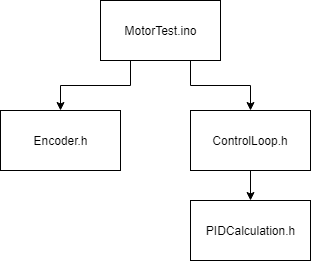
\includegraphics[width=6 cm]{MotorcontrollerArchitecture.png}
\caption{Motorcontroller architecture.}
\label{fig::Motorconarc}
\end{figure}

\subsection{Arduino Mega Code}
The main program combines the classes together. It will also send the commands to the actual motor controller via serial bus. The commands send to the motor are refreshed at a higher frequency than the control loop is called. The flow of the main program can be found in figure \ref{fig::MPF}.

\begin{figure}[H]
\centering
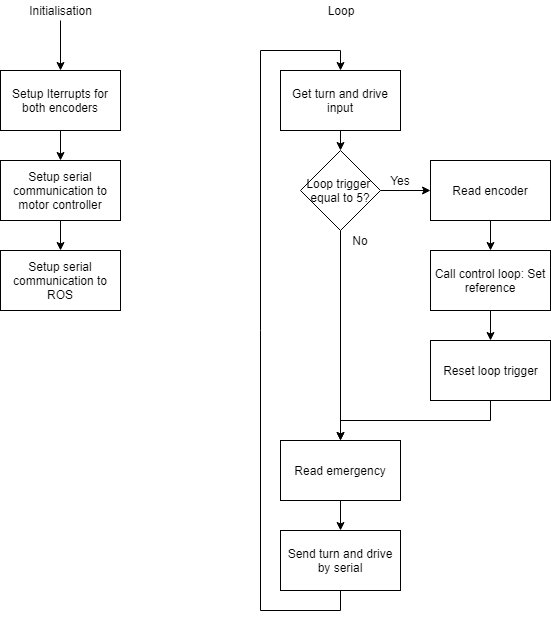
\includegraphics[width=12 cm]{MainProgramFlow.png}
\caption{Main program flow.}
\label{fig::MPF}
\end{figure}


\subsection{Rotary encoders}
The rotary encoders are of the quadrature type with 256 PPR. 
Quadruature encoders are equiped with two channels from which one is phase shifted 90 degrees over the other, see figure \ref{fig::QuadEnc}.
This allows to determine the direction in which the shaft is rotating and to increase resolution.

\begin{figure}[H]
\centering
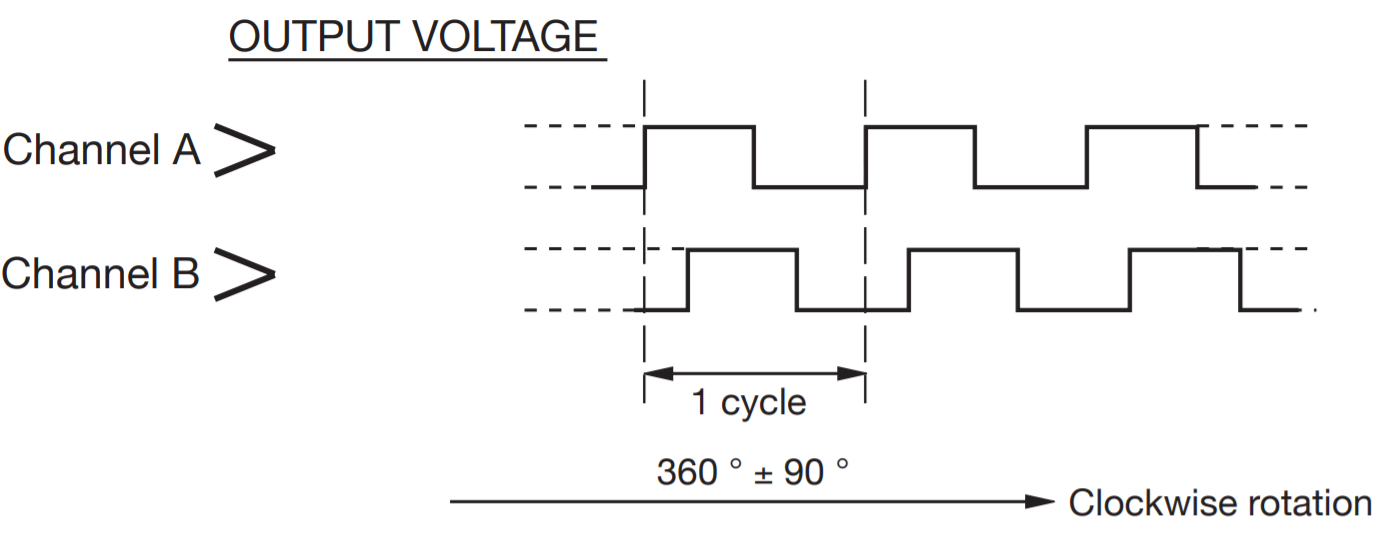
\includegraphics[width=12 cm]{QuadruatureEncoderOutput.png}
\caption{Output from quardature encoder.}
\label{fig::QuadEnc}
\end{figure}


Interrupts are generated for the rising egde an for the falling egde on the puls train per channel and therefore increase the resolution to 1024 per revolution. 
The speed is determined using the analogy which can be found in the the two flowcharts below. The interrupts will trigger the direction determination and call an puls change function which stores timestamps and calculation of periods. This can be found in figure \ref{fig::PCF}.

When the main program wants to now the speed, it will call a speed read function which will then calculate the speed accordingly. This can be found in figure \ref{fig::SRC}.

\begin{figure}[H]
\centering
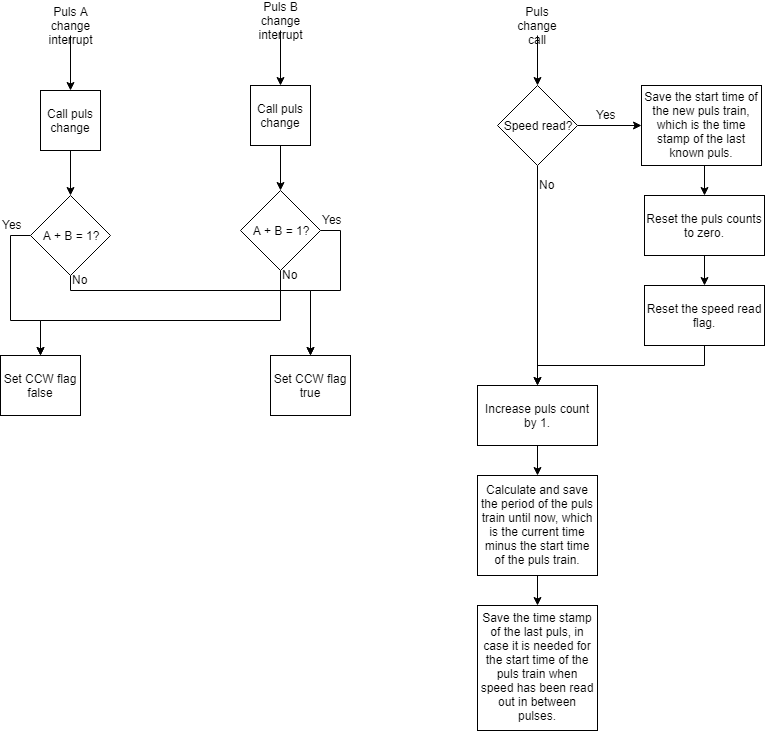
\includegraphics[width=16 cm]{Speed_determinator-Page-1.png}
\caption{Puls change interrupt flow.}
\label{fig::PCF}
\end{figure}


\begin{figure}[H]
\centering
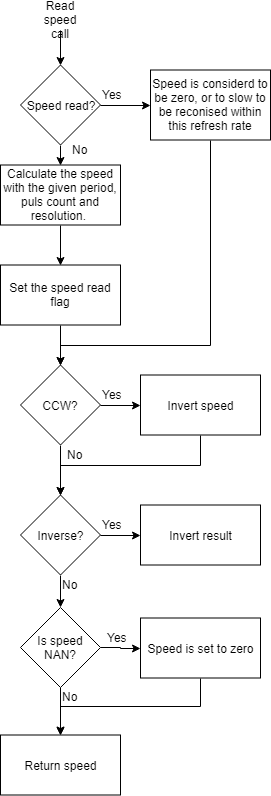
\includegraphics[width=6 cm]{Speed_determinator-Page-2.png}
\caption{Speed read call.}
\label{fig::SRC}
\end{figure}

\subsection{Control loop}
The control loop calculates the speed error per wheel based on feedback of the encoders and a reference turn and drive input. 
This error is send to the PIDCalculation which returns a turn and drive output. 
A detailed description of these calculations can be found in movement research. 
The flow of this class can be found in figure \ref{fig::CLF}.

\begin{figure}[H]
\centering
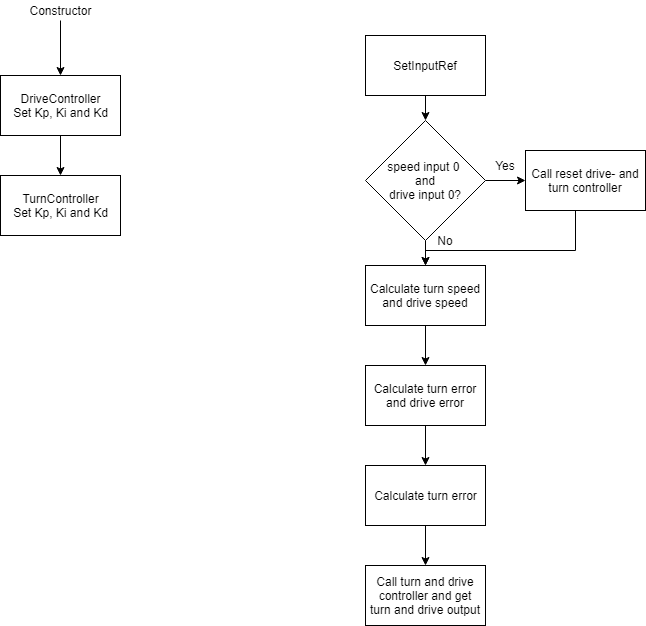
\includegraphics[width=6 cm]{ControlLoop.png}
\caption{Control loop flow.}
\label{fig::CLF}
\end{figure}

